\documentclass[1p]{elsarticle_modified}
%\bibliographystyle{elsarticle-num}

%\usepackage[colorlinks]{hyperref}
%\usepackage{abbrmath_seonhwa} %\Abb, \Ascr, \Acal ,\Abf, \Afrak
\usepackage{amsfonts}
\usepackage{amssymb}
\usepackage{amsmath}
\usepackage{amsthm}
\usepackage{scalefnt}
\usepackage{amsbsy}
\usepackage{kotex}
\usepackage{caption}
\usepackage{subfig}
\usepackage{color}
\usepackage{graphicx}
\usepackage{xcolor} %% white, black, red, green, blue, cyan, magenta, yellow
\usepackage{float}
\usepackage{setspace}
\usepackage{hyperref}

\usepackage{tikz}
\usetikzlibrary{arrows}

\usepackage{multirow}
\usepackage{array} % fixed length table
\usepackage{hhline}

%%%%%%%%%%%%%%%%%%%%%
\makeatletter
\renewcommand*\env@matrix[1][\arraystretch]{%
	\edef\arraystretch{#1}%
	\hskip -\arraycolsep
	\let\@ifnextchar\new@ifnextchar
	\array{*\c@MaxMatrixCols c}}
\makeatother %https://tex.stackexchange.com/questions/14071/how-can-i-increase-the-line-spacing-in-a-matrix
%%%%%%%%%%%%%%%

\usepackage[normalem]{ulem}

\newcommand{\msout}[1]{\ifmmode\text{\sout{\ensuremath{#1}}}\else\sout{#1}\fi}
%SOURCE: \msout is \stkout macro in https://tex.stackexchange.com/questions/20609/strikeout-in-math-mode

\newcommand{\cancel}[1]{
	\ifmmode
	{\color{red}\msout{#1}}
	\else
	{\color{red}\sout{#1}}
	\fi
}

\newcommand{\add}[1]{
	{\color{blue}\uwave{#1}}
}

\newcommand{\replace}[2]{
	\ifmmode
	{\color{red}\msout{#1}}{\color{blue}\uwave{#2}}
	\else
	{\color{red}\sout{#1}}{\color{blue}\uwave{#2}}
	\fi
}

\newcommand{\Sol}{\mathcal{S}} %segment
\newcommand{\D}{D} %diagram
\newcommand{\A}{\mathcal{A}} %arc


%%%%%%%%%%%%%%%%%%%%%%%%%%%%%5 test

\def\sl{\operatorname{\textup{SL}}(2,\Cbb)}
\def\psl{\operatorname{\textup{PSL}}(2,\Cbb)}
\def\quan{\mkern 1mu \triangleright \mkern 1mu}

\theoremstyle{definition}
\newtheorem{thm}{Theorem}[section]
\newtheorem{prop}[thm]{Proposition}
\newtheorem{lem}[thm]{Lemma}
\newtheorem{ques}[thm]{Question}
\newtheorem{cor}[thm]{Corollary}
\newtheorem{defn}[thm]{Definition}
\newtheorem{exam}[thm]{Example}
\newtheorem{rmk}[thm]{Remark}
\newtheorem{alg}[thm]{Algorithm}

\newcommand{\I}{\sqrt{-1}}
\begin{document}

%\begin{frontmatter}
%
%\title{Boundary parabolic representations of knots up to 8 crossings}
%
%%% Group authors per affiliation:
%\author{Yunhi Cho} 
%\address{Department of Mathematics, University of Seoul, Seoul, Korea}
%\ead{yhcho@uos.ac.kr}
%
%
%\author{Seonhwa Kim} %\fnref{s_kim}}
%\address{Center for Geometry and Physics, Institute for Basic Science, Pohang, 37673, Korea}
%\ead{ryeona17@ibs.re.kr}
%
%\author{Hyuk Kim}
%\address{Department of Mathematical Sciences, Seoul National University, Seoul 08826, Korea}
%\ead{hyukkim@snu.ac.kr}
%
%\author{Seokbeom Yoon}
%\address{Department of Mathematical Sciences, Seoul National University, Seoul, 08826,  Korea}
%\ead{sbyoon15@snu.ac.kr}
%
%\begin{abstract}
%We find all boundary parabolic representation of knots up to 8 crossings.
%
%\end{abstract}
%\begin{keyword}
%    \MSC[2010] 57M25 
%\end{keyword}
%
%\end{frontmatter}

%\linenumbers
%\tableofcontents
%
\newcommand\colored[1]{\textcolor{white}{\rule[-0.35ex]{0.8em}{1.4ex}}\kern-0.8em\color{red} #1}%
%\newcommand\colored[1]{\textcolor{white}{ #1}\kern-2.17ex	\textcolor{white}{ #1}\kern-1.81ex	\textcolor{white}{ #1}\kern-2.15ex\color{red}#1	}

{\Large $\underline{12n_{0688}~(K12n_{0688})}$}

\setlength{\tabcolsep}{10pt}
\renewcommand{\arraystretch}{1.6}
\vspace{1cm}\begin{tabular}{m{100pt}>{\centering\arraybackslash}m{274pt}}
\multirow{5}{120pt}{
	\centering
	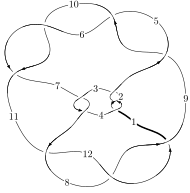
\includegraphics[width=112pt]{../../../GIT/diagram.site/Diagrams/png/2777_12n_0688.png}\\
\ \ \ A knot diagram\footnotemark}&
\allowdisplaybreaks
\textbf{Linearized knot diagam} \\
\cline{2-2}
 &
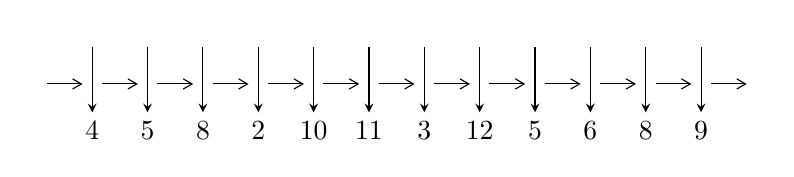
\begin{tikzpicture}[x=20pt, y=17pt]
	% nodes
	\node (C0) at (0, 0) {};
	\node (C1) at (1, 0) {};
	\node (C1U) at (1, +1) {};
	\node (C1D) at (1, -1) {4};

	\node (C2) at (2, 0) {};
	\node (C2U) at (2, +1) {};
	\node (C2D) at (2, -1) {5};

	\node (C3) at (3, 0) {};
	\node (C3U) at (3, +1) {};
	\node (C3D) at (3, -1) {8};

	\node (C4) at (4, 0) {};
	\node (C4U) at (4, +1) {};
	\node (C4D) at (4, -1) {2};

	\node (C5) at (5, 0) {};
	\node (C5U) at (5, +1) {};
	\node (C5D) at (5, -1) {10};

	\node (C6) at (6, 0) {};
	\node (C6U) at (6, +1) {};
	\node (C6D) at (6, -1) {11};

	\node (C7) at (7, 0) {};
	\node (C7U) at (7, +1) {};
	\node (C7D) at (7, -1) {3};

	\node (C8) at (8, 0) {};
	\node (C8U) at (8, +1) {};
	\node (C8D) at (8, -1) {12};

	\node (C9) at (9, 0) {};
	\node (C9U) at (9, +1) {};
	\node (C9D) at (9, -1) {5};

	\node (C10) at (10, 0) {};
	\node (C10U) at (10, +1) {};
	\node (C10D) at (10, -1) {6};

	\node (C11) at (11, 0) {};
	\node (C11U) at (11, +1) {};
	\node (C11D) at (11, -1) {8};

	\node (C12) at (12, 0) {};
	\node (C12U) at (12, +1) {};
	\node (C12D) at (12, -1) {9};
	\node (C13) at (13, 0) {};

	% arrows
	\draw[->,>={angle 60}]
	(C0) edge (C1) (C1) edge (C2) (C2) edge (C3) (C3) edge (C4) (C4) edge (C5) (C5) edge (C6) (C6) edge (C7) (C7) edge (C8) (C8) edge (C9) (C9) edge (C10) (C10) edge (C11) (C11) edge (C12) (C12) edge (C13) ;	\draw[->,>=stealth]
	(C1U) edge (C1D) (C2U) edge (C2D) (C3U) edge (C3D) (C4U) edge (C4D) (C5U) edge (C5D) (C6U) edge (C6D) (C7U) edge (C7D) (C8U) edge (C8D) (C9U) edge (C9D) (C10U) edge (C10D) (C11U) edge (C11D) (C12U) edge (C12D) ;
	\end{tikzpicture} \\
\hhline{~~} \\& 
\textbf{Solving Sequence} \\ \cline{2-2} 
 &
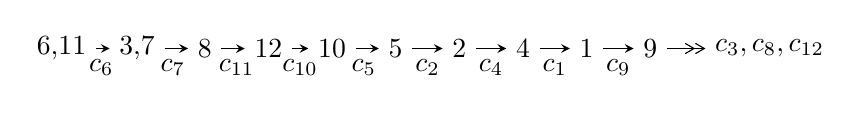
\begin{tikzpicture}[x=23pt, y=7pt]
	% node
	\node (A0) at (-1/8, 0) {6,11};
	\node (A1) at (17/16, 0) {3,7};
	\node (A2) at (17/8, 0) {8};
	\node (A3) at (25/8, 0) {12};
	\node (A4) at (33/8, 0) {10};
	\node (A5) at (41/8, 0) {5};
	\node (A6) at (49/8, 0) {2};
	\node (A7) at (57/8, 0) {4};
	\node (A8) at (65/8, 0) {1};
	\node (A9) at (73/8, 0) {9};
	\node (C1) at (1/2, -1) {$c_{6}$};
	\node (C2) at (13/8, -1) {$c_{7}$};
	\node (C3) at (21/8, -1) {$c_{11}$};
	\node (C4) at (29/8, -1) {$c_{10}$};
	\node (C5) at (37/8, -1) {$c_{5}$};
	\node (C6) at (45/8, -1) {$c_{2}$};
	\node (C7) at (53/8, -1) {$c_{4}$};
	\node (C8) at (61/8, -1) {$c_{1}$};
	\node (C9) at (69/8, -1) {$c_{9}$};
	\node (A10) at (11, 0) {$c_{3},c_{8},c_{12}$};

	% edge
	\draw[->,>=stealth]	
	(A0) edge (A1) (A1) edge (A2) (A2) edge (A3) (A3) edge (A4) (A4) edge (A5) (A5) edge (A6) (A6) edge (A7) (A7) edge (A8) (A8) edge (A9) ;
	\draw[->>,>={angle 60}]	
	(A9) edge (A10);
\end{tikzpicture} \\ 

\end{tabular} \\

\footnotetext{
The image of knot diagram is generated by the software ``\textbf{Draw programme}" developed by Andrew Bartholomew(\url{http://www.layer8.co.uk/maths/draw/index.htm\#Running-draw}), where we modified some parts for our purpose(\url{https://github.com/CATsTAILs/LinksPainter}).
}\phantom \\ \newline 
\centering \textbf{Ideals for irreducible components\footnotemark of $X_{\text{par}}$} 
 
\begin{align*}
I^u_{1}&=\langle 
-1.45733\times10^{20} u^{26}-2.14063\times10^{20} u^{25}+\cdots+3.64969\times10^{20} b+1.19460\times10^{21},\\
\phantom{I^u_{1}}&\phantom{= \langle  }-4.51116\times10^{20} u^{26}-7.95319\times10^{20} u^{25}+\cdots+3.64969\times10^{20} a+5.99946\times10^{21},\\
\phantom{I^u_{1}}&\phantom{= \langle  }u^{27}+2 u^{26}+\cdots-12 u-4\rangle \\
I^u_{2}&=\langle 
b- u+1,\;- u^2+a+3,\;u^3- u^2-2 u+1\rangle \\
I^u_{3}&=\langle 
- a u+b+1,\;2 a^2+a u+2 a-2 u-3,\;u^2-2\rangle \\
\\
I^v_{1}&=\langle 
a,\;b- v-2,\;v^2+3 v+1\rangle \\
\end{align*}
\raggedright * 4 irreducible components of $\dim_{\mathbb{C}}=0$, with total 36 representations.\\
\footnotetext{All coefficients of polynomials are rational numbers. But the coefficients are sometimes approximated in decimal forms when there is not enough margin.}
\newpage
\renewcommand{\arraystretch}{1}
\centering \section*{I. $I^u_{1}= \langle -1.46\times10^{20} u^{26}-2.14\times10^{20} u^{25}+\cdots+3.65\times10^{20} b+1.19\times10^{21},\;-4.51\times10^{20} u^{26}-7.95\times10^{20} u^{25}+\cdots+3.65\times10^{20} a+6.00\times10^{21},\;u^{27}+2 u^{26}+\cdots-12 u-4 \rangle$}
\flushleft \textbf{(i) Arc colorings}\\
\begin{tabular}{m{7pt} m{180pt} m{7pt} m{180pt} }
\flushright $a_{6}=$&$\begin{pmatrix}1\\0\end{pmatrix}$ \\
\flushright $a_{11}=$&$\begin{pmatrix}0\\u\end{pmatrix}$ \\
\flushright $a_{3}=$&$\begin{pmatrix}1.23604 u^{26}+2.17914 u^{25}+\cdots+8.25237 u-16.4383\\0.399304 u^{26}+0.586525 u^{25}+\cdots-3.39246 u-3.27317\end{pmatrix}$ \\
\flushright $a_{7}=$&$\begin{pmatrix}1\\u^2\end{pmatrix}$ \\
\flushright $a_{8}=$&$\begin{pmatrix}0.738918 u^{26}+1.22294 u^{25}+\cdots+2.14974 u-8.57454\\0.353041 u^{26}+0.631631 u^{25}+\cdots-2.16585 u-3.44416\end{pmatrix}$ \\
\flushright $a_{12}=$&$\begin{pmatrix}0.175121 u^{26}+0.148966 u^{25}+\cdots-7.10327 u+0.964438\\0.560998 u^{26}+0.740275 u^{25}+\cdots-2.78768 u-4.16594\end{pmatrix}$ \\
\flushright $a_{10}=$&$\begin{pmatrix}u\\u\end{pmatrix}$ \\
\flushright $a_{5}=$&$\begin{pmatrix}- u^2+1\\- u^2\end{pmatrix}$ \\
\flushright $a_{2}=$&$\begin{pmatrix}1.66235 u^{26}+2.73772 u^{25}+\cdots+6.10273 u-20.0632\\0.563386 u^{26}+0.613561 u^{25}+\cdots-4.52635 u-3.30149\end{pmatrix}$ \\
\flushright $a_{4}=$&$\begin{pmatrix}0.670706 u^{26}+1.16883 u^{25}+\cdots+9.64782 u-9.46907\\-0.635285 u^{26}-0.677229 u^{25}+\cdots+4.25702 u+3.47590\end{pmatrix}$ \\
\flushright $a_{1}=$&$\begin{pmatrix}-0.0973141 u^{26}+0.0651568 u^{25}+\cdots+7.52379 u-2.64979\\-0.591878 u^{26}-0.655073 u^{25}+\cdots+3.31129 u+3.50017\end{pmatrix}$ \\
\flushright $a_{9}=$&$\begin{pmatrix}- u^3+2 u\\- u^3+u\end{pmatrix}$\\&\end{tabular}
\flushleft \textbf{(ii) Obstruction class $= -1$}\\~\\
\flushleft \textbf{(iii) Cusp Shapes $= \frac{237495891437804361646}{91242178035245717881} u^{26}+\frac{405928781365325849828}{91242178035245717881} u^{25}+\cdots+\frac{4084274379373058773658}{91242178035245717881} u-\frac{5388560215252919173048}{91242178035245717881}$}\\~\\
\newpage\renewcommand{\arraystretch}{1}
\flushleft \textbf{(iv) u-Polynomials at the component}\newline \\
\begin{tabular}{m{50pt}|m{274pt}}
Crossings & \hspace{64pt}u-Polynomials at each crossing \\
\hline $$\begin{aligned}c_{1},c_{2},c_{4}\end{aligned}$$&$\begin{aligned}
&u^{27}-7 u^{26}+\cdots-9 u-1
\end{aligned}$\\
\hline $$\begin{aligned}c_{3},c_{7}\end{aligned}$$&$\begin{aligned}
&u^{27}-2 u^{26}+\cdots-52 u+8
\end{aligned}$\\
\hline $$\begin{aligned}c_{5},c_{6},c_{9}\\c_{10}\end{aligned}$$&$\begin{aligned}
&u^{27}-2 u^{26}+\cdots-12 u+4
\end{aligned}$\\
\hline $$\begin{aligned}c_{8},c_{11},c_{12}\end{aligned}$$&$\begin{aligned}
&u^{27}+4 u^{26}+\cdots-57 u-9
\end{aligned}$\\
\hline
\end{tabular}\\~\\
\newpage\renewcommand{\arraystretch}{1}
\flushleft \textbf{(v) Riley Polynomials at the component}\newline \\
\begin{tabular}{m{50pt}|m{274pt}}
Crossings & \hspace{64pt}Riley Polynomials at each crossing \\
\hline $$\begin{aligned}c_{1},c_{2},c_{4}\end{aligned}$$&$\begin{aligned}
&y^{27}-15 y^{26}+\cdots+103 y-1
\end{aligned}$\\
\hline $$\begin{aligned}c_{3},c_{7}\end{aligned}$$&$\begin{aligned}
&y^{27}+12 y^{26}+\cdots+3920 y-64
\end{aligned}$\\
\hline $$\begin{aligned}c_{5},c_{6},c_{9}\\c_{10}\end{aligned}$$&$\begin{aligned}
&y^{27}-24 y^{26}+\cdots+432 y-16
\end{aligned}$\\
\hline $$\begin{aligned}c_{8},c_{11},c_{12}\end{aligned}$$&$\begin{aligned}
&y^{27}-10 y^{26}+\cdots+1179 y-81
\end{aligned}$\\
\hline
\end{tabular}\\~\\
\newpage\flushleft \textbf{(vi) Complex Volumes and Cusp Shapes}
$$\begin{array}{c|c|c}  
\text{Solutions to }I^u_{1}& \I (\text{vol} + \sqrt{-1}CS) & \text{Cusp shape}\\
 \hline 
\begin{aligned}
u &= -0.103210 + 1.061510 I \\
a &= \phantom{-}0.243591 + 1.283730 I \\
b &= \phantom{-}0.314942 + 0.159811 I\end{aligned}
 & \phantom{-}5.33632 - 0.36665 I & -12.32525 - 0.05039 I \\ \hline\begin{aligned}
u &= -0.103210 - 1.061510 I \\
a &= \phantom{-}0.243591 - 1.283730 I \\
b &= \phantom{-}0.314942 - 0.159811 I\end{aligned}
 & \phantom{-}5.33632 + 0.36665 I & -12.32525 + 0.05039 I \\ \hline\begin{aligned}
u &= -0.903239 + 0.167691 I \\
a &= -1.45135 - 0.68497 I \\
b &= -0.485625 - 0.865359 I\end{aligned}
 & -3.12027 + 0.78467 I & -18.4367 - 3.3729 I \\ \hline\begin{aligned}
u &= -0.903239 - 0.167691 I \\
a &= -1.45135 + 0.68497 I \\
b &= -0.485625 + 0.865359 I\end{aligned}
 & -3.12027 - 0.78467 I & -18.4367 + 3.3729 I \\ \hline\begin{aligned}
u &= \phantom{-}0.337221 + 1.048840 I \\
a &= \phantom{-}0.052763 - 1.351640 I \\
b &= \phantom{-}0.215415 - 0.194118 I\end{aligned}
 & \phantom{-}3.59374 - 7.31725 I & -14.7365 + 5.0472 I \\ \hline\begin{aligned}
u &= \phantom{-}0.337221 - 1.048840 I \\
a &= \phantom{-}0.052763 + 1.351640 I \\
b &= \phantom{-}0.215415 + 0.194118 I\end{aligned}
 & \phantom{-}3.59374 + 7.31725 I & -14.7365 - 5.0472 I \\ \hline\begin{aligned}
u &= \phantom{-}1.104930 + 0.368271 I \\
a &= -0.268980 + 0.135914 I \\
b &= \phantom{-}0.714285 - 1.043610 I\end{aligned}
 & -3.05220 - 3.96537 I & -17.7910 + 4.2991 I \\ \hline\begin{aligned}
u &= \phantom{-}1.104930 - 0.368271 I \\
a &= -0.268980 - 0.135914 I \\
b &= \phantom{-}0.714285 + 1.043610 I\end{aligned}
 & -3.05220 + 3.96537 I & -17.7910 - 4.2991 I \\ \hline\begin{aligned}
u &= \phantom{-}1.020210 + 0.720557 I \\
a &= \phantom{-}0.780740 - 0.476181 I \\
b &= \phantom{-}1.045480 - 0.589623 I\end{aligned}
 & \phantom{-}1.52420 + 1.21028 I & -14.6857 - 1.0471 I \\ \hline\begin{aligned}
u &= \phantom{-}1.020210 - 0.720557 I \\
a &= \phantom{-}0.780740 + 0.476181 I \\
b &= \phantom{-}1.045480 + 0.589623 I\end{aligned}
 & \phantom{-}1.52420 - 1.21028 I & -14.6857 + 1.0471 I\\
 \hline 
 \end{array}$$\newpage$$\begin{array}{c|c|c}  
\text{Solutions to }I^u_{1}& \I (\text{vol} + \sqrt{-1}CS) & \text{Cusp shape}\\
 \hline 
\begin{aligned}
u &= -1.33719\phantom{ +0.000000I} \\
a &= \phantom{-}0.790731\phantom{ +0.000000I} \\
b &= -0.340332\phantom{ +0.000000I}\end{aligned}
 & -14.1221\phantom{ +0.000000I} & -16.5250\phantom{ +0.000000I} \\ \hline\begin{aligned}
u &= -1.374500 + 0.240422 I \\
a &= -0.496066 - 0.228689 I \\
b &= -1.169080 - 0.741326 I\end{aligned}
 & -6.49373 + 0.53770 I & -14.7868 - 0.8041 I \\ \hline\begin{aligned}
u &= -1.374500 - 0.240422 I \\
a &= -0.496066 + 0.228689 I \\
b &= -1.169080 + 0.741326 I\end{aligned}
 & -6.49373 - 0.53770 I & -14.7868 + 0.8041 I \\ \hline\begin{aligned}
u &= \phantom{-}1.40105\phantom{ +0.000000I} \\
a &= -11.6087\phantom{ +0.000000I} \\
b &= -22.6375\phantom{ +0.000000I}\end{aligned}
 & -8.19904\phantom{ +0.000000I} & -208.640\phantom{ +0.000000I} \\ \hline\begin{aligned}
u &= -1.295330 + 0.551421 I \\
a &= \phantom{-}0.862994 + 0.773421 I \\
b &= \phantom{-}1.25669 + 1.17478 I\end{aligned}
 & \phantom{-}1.64132 + 6.06050 I & -15.3648 - 4.1353 I \\ \hline\begin{aligned}
u &= -1.295330 - 0.551421 I \\
a &= \phantom{-}0.862994 - 0.773421 I \\
b &= \phantom{-}1.25669 - 1.17478 I\end{aligned}
 & \phantom{-}1.64132 - 6.06050 I & -15.3648 + 4.1353 I \\ \hline\begin{aligned}
u &= \phantom{-}0.279491 + 0.475963 I \\
a &= \phantom{-}0.278696 - 0.748546 I \\
b &= -0.794845 + 0.094176 I\end{aligned}
 & -0.648673 + 0.468512 I & -12.96489 + 0.08688 I \\ \hline\begin{aligned}
u &= \phantom{-}0.279491 - 0.475963 I \\
a &= \phantom{-}0.278696 + 0.748546 I \\
b &= -0.794845 - 0.094176 I\end{aligned}
 & -0.648673 - 0.468512 I & -12.96489 - 0.08688 I \\ \hline\begin{aligned}
u &= -1.45969\phantom{ +0.000000I} \\
a &= -1.05208\phantom{ +0.000000I} \\
b &= -1.81866\phantom{ +0.000000I}\end{aligned}
 & -6.73578\phantom{ +0.000000I} & -12.1710\phantom{ +0.000000I} \\ \hline\begin{aligned}
u &= \phantom{-}1.44790 + 0.52184 I \\
a &= -0.710802 + 0.417384 I \\
b &= -1.42465 + 1.21712 I\end{aligned}
 & \phantom{-}0.46040 - 5.31882 I & -15.6377 + 3.3723 I\\
 \hline 
 \end{array}$$\newpage$$\begin{array}{c|c|c}  
\text{Solutions to }I^u_{1}& \I (\text{vol} + \sqrt{-1}CS) & \text{Cusp shape}\\
 \hline 
\begin{aligned}
u &= \phantom{-}1.44790 - 0.52184 I \\
a &= -0.710802 - 0.417384 I \\
b &= -1.42465 - 1.21712 I\end{aligned}
 & \phantom{-}0.46040 + 5.31882 I & -15.6377 - 3.3723 I \\ \hline\begin{aligned}
u &= -0.459185\phantom{ +0.000000I} \\
a &= \phantom{-}1.01896\phantom{ +0.000000I} \\
b &= \phantom{-}1.69587\phantom{ +0.000000I}\end{aligned}
 & -10.8656\phantom{ +0.000000I} & -30.2970\phantom{ +0.000000I} \\ \hline\begin{aligned}
u &= -1.51780 + 0.43184 I \\
a &= -0.849204 - 0.755740 I \\
b &= -1.65455 - 1.79207 I\end{aligned}
 & -2.32586 + 12.67780 I & -18.7053 - 6.5054 I \\ \hline\begin{aligned}
u &= -1.51780 - 0.43184 I \\
a &= -0.849204 + 0.755740 I \\
b &= -1.65455 + 1.79207 I\end{aligned}
 & -2.32586 - 12.67780 I & -18.7053 + 6.5054 I \\ \hline\begin{aligned}
u &= \phantom{-}0.379857\phantom{ +0.000000I} \\
a &= \phantom{-}0.653894\phantom{ +0.000000I} \\
b &= -0.255787\phantom{ +0.000000I}\end{aligned}
 & -0.575852\phantom{ +0.000000I} & -17.0320\phantom{ +0.000000I} \\ \hline\begin{aligned}
u &= -0.278308\phantom{ +0.000000I} \\
a &= -8.72003\phantom{ +0.000000I} \\
b &= -0.183695\phantom{ +0.000000I}\end{aligned}
 & -2.85525\phantom{ +0.000000I} & -50.3790\phantom{ +0.000000I} \\ \hline\begin{aligned}
u &= \phantom{-}1.76214\phantom{ +0.000000I} \\
a &= \phantom{-}0.0324794\phantom{ +0.000000I} \\
b &= -0.496020\phantom{ +0.000000I}\end{aligned}
 & -19.5641\phantom{ +0.000000I} & -33.0880\phantom{ +0.000000I}\\
 \hline 
 \end{array}$$\newpage\newpage\renewcommand{\arraystretch}{1}
\centering \section*{II. $I^u_{2}= \langle b- u+1,\;- u^2+a+3,\;u^3- u^2-2 u+1 \rangle$}
\flushleft \textbf{(i) Arc colorings}\\
\begin{tabular}{m{7pt} m{180pt} m{7pt} m{180pt} }
\flushright $a_{6}=$&$\begin{pmatrix}1\\0\end{pmatrix}$ \\
\flushright $a_{11}=$&$\begin{pmatrix}0\\u\end{pmatrix}$ \\
\flushright $a_{3}=$&$\begin{pmatrix}u^2-3\\u-1\end{pmatrix}$ \\
\flushright $a_{7}=$&$\begin{pmatrix}1\\u^2\end{pmatrix}$ \\
\flushright $a_{8}=$&$\begin{pmatrix}1\\u^2\end{pmatrix}$ \\
\flushright $a_{12}=$&$\begin{pmatrix}- u\\- u^2- u+1\end{pmatrix}$ \\
\flushright $a_{10}=$&$\begin{pmatrix}u\\u\end{pmatrix}$ \\
\flushright $a_{5}=$&$\begin{pmatrix}- u^2+1\\- u^2\end{pmatrix}$ \\
\flushright $a_{2}=$&$\begin{pmatrix}2 u^2-4\\u^2+u-1\end{pmatrix}$ \\
\flushright $a_{4}=$&$\begin{pmatrix}u^2-3\\u-1\end{pmatrix}$ \\
\flushright $a_{1}=$&$\begin{pmatrix}u^2-1\\u^2\end{pmatrix}$ \\
\flushright $a_{9}=$&$\begin{pmatrix}- u^2+1\\- u^2- u+1\end{pmatrix}$\\&\end{tabular}
\flushleft \textbf{(ii) Obstruction class $= 1$}\\~\\
\flushleft \textbf{(iii) Cusp Shapes $= u^2+4 u-16$}\\~\\
\newpage\renewcommand{\arraystretch}{1}
\flushleft \textbf{(iv) u-Polynomials at the component}\newline \\
\begin{tabular}{m{50pt}|m{274pt}}
Crossings & \hspace{64pt}u-Polynomials at each crossing \\
\hline $$\begin{aligned}c_{1},c_{2}\end{aligned}$$&$\begin{aligned}
&(u-1)^3
\end{aligned}$\\
\hline $$\begin{aligned}c_{3},c_{7}\end{aligned}$$&$\begin{aligned}
&u^3
\end{aligned}$\\
\hline $$\begin{aligned}c_{4}\end{aligned}$$&$\begin{aligned}
&(u+1)^3
\end{aligned}$\\
\hline $$\begin{aligned}c_{5},c_{6},c_{8}\end{aligned}$$&$\begin{aligned}
&u^3- u^2-2 u+1
\end{aligned}$\\
\hline $$\begin{aligned}c_{9},c_{10},c_{11}\\c_{12}\end{aligned}$$&$\begin{aligned}
&u^3+u^2-2 u-1
\end{aligned}$\\
\hline
\end{tabular}\\~\\
\newpage\renewcommand{\arraystretch}{1}
\flushleft \textbf{(v) Riley Polynomials at the component}\newline \\
\begin{tabular}{m{50pt}|m{274pt}}
Crossings & \hspace{64pt}Riley Polynomials at each crossing \\
\hline $$\begin{aligned}c_{1},c_{2},c_{4}\end{aligned}$$&$\begin{aligned}
&(y-1)^3
\end{aligned}$\\
\hline $$\begin{aligned}c_{3},c_{7}\end{aligned}$$&$\begin{aligned}
&y^3
\end{aligned}$\\
\hline $$\begin{aligned}c_{5},c_{6},c_{8}\\c_{9},c_{10},c_{11}\\c_{12}\end{aligned}$$&$\begin{aligned}
&y^3-5 y^2+6 y-1
\end{aligned}$\\
\hline
\end{tabular}\\~\\
\newpage\flushleft \textbf{(vi) Complex Volumes and Cusp Shapes}
$$\begin{array}{c|c|c}  
\text{Solutions to }I^u_{2}& \I (\text{vol} + \sqrt{-1}CS) & \text{Cusp shape}\\
 \hline 
\begin{aligned}
u &= -1.24698\phantom{ +0.000000I} \\
a &= -1.44504\phantom{ +0.000000I} \\
b &= -2.24698\phantom{ +0.000000I}\end{aligned}
 & -7.98968\phantom{ +0.000000I} & -19.4330\phantom{ +0.000000I} \\ \hline\begin{aligned}
u &= \phantom{-}0.445042\phantom{ +0.000000I} \\
a &= -2.80194\phantom{ +0.000000I} \\
b &= -0.554958\phantom{ +0.000000I}\end{aligned}
 & -2.34991\phantom{ +0.000000I} & -14.0220\phantom{ +0.000000I} \\ \hline\begin{aligned}
u &= \phantom{-}1.80194\phantom{ +0.000000I} \\
a &= \phantom{-}0.246980\phantom{ +0.000000I} \\
b &= \phantom{-}0.801938\phantom{ +0.000000I}\end{aligned}
 & -19.2692\phantom{ +0.000000I} & -5.54530\phantom{ +0.000000I}\\
 \hline 
 \end{array}$$\newpage\newpage\renewcommand{\arraystretch}{1}
\centering \section*{III. $I^u_{3}= \langle - a u+b+1,\;2 a^2+a u+2 a-2 u-3,\;u^2-2 \rangle$}
\flushleft \textbf{(i) Arc colorings}\\
\begin{tabular}{m{7pt} m{180pt} m{7pt} m{180pt} }
\flushright $a_{6}=$&$\begin{pmatrix}1\\0\end{pmatrix}$ \\
\flushright $a_{11}=$&$\begin{pmatrix}0\\u\end{pmatrix}$ \\
\flushright $a_{3}=$&$\begin{pmatrix}a\\a u-1\end{pmatrix}$ \\
\flushright $a_{7}=$&$\begin{pmatrix}1\\2\end{pmatrix}$ \\
\flushright $a_{8}=$&$\begin{pmatrix}-\frac{1}{2} u\\- a u+2 a- u+2\end{pmatrix}$ \\
\flushright $a_{12}=$&$\begin{pmatrix}-\frac{1}{2} u\\- a u+2 a+2\end{pmatrix}$ \\
\flushright $a_{10}=$&$\begin{pmatrix}u\\u\end{pmatrix}$ \\
\flushright $a_{5}=$&$\begin{pmatrix}-1\\-2\end{pmatrix}$ \\
\flushright $a_{2}=$&$\begin{pmatrix}a u- a-1\\3 a u-4 a-3\end{pmatrix}$ \\
\flushright $a_{4}=$&$\begin{pmatrix}- a u+2 a-\frac{1}{2} u\\-3 a u+6 a- u+2\end{pmatrix}$ \\
\flushright $a_{1}=$&$\begin{pmatrix}-\frac{1}{2} u\\- a u+2 a- u+2\end{pmatrix}$ \\
\flushright $a_{9}=$&$\begin{pmatrix}0\\- u\end{pmatrix}$\\&\end{tabular}
\flushleft \textbf{(ii) Obstruction class $= 1$}\\~\\
\flushleft \textbf{(iii) Cusp Shapes $= -24$}\\~\\
\newpage\renewcommand{\arraystretch}{1}
\flushleft \textbf{(iv) u-Polynomials at the component}\newline \\
\begin{tabular}{m{50pt}|m{274pt}}
Crossings & \hspace{64pt}u-Polynomials at each crossing \\
\hline $$\begin{aligned}c_{1},c_{2},c_{7}\end{aligned}$$&$\begin{aligned}
&(u^2+u-1)^2
\end{aligned}$\\
\hline $$\begin{aligned}c_{3},c_{4}\end{aligned}$$&$\begin{aligned}
&(u^2- u-1)^2
\end{aligned}$\\
\hline $$\begin{aligned}c_{5},c_{6},c_{9}\\c_{10}\end{aligned}$$&$\begin{aligned}
&(u^2-2)^2
\end{aligned}$\\
\hline $$\begin{aligned}c_{8}\end{aligned}$$&$\begin{aligned}
&(u+1)^4
\end{aligned}$\\
\hline $$\begin{aligned}c_{11},c_{12}\end{aligned}$$&$\begin{aligned}
&(u-1)^4
\end{aligned}$\\
\hline
\end{tabular}\\~\\
\newpage\renewcommand{\arraystretch}{1}
\flushleft \textbf{(v) Riley Polynomials at the component}\newline \\
\begin{tabular}{m{50pt}|m{274pt}}
Crossings & \hspace{64pt}Riley Polynomials at each crossing \\
\hline $$\begin{aligned}c_{1},c_{2},c_{3}\\c_{4},c_{7}\end{aligned}$$&$\begin{aligned}
&(y^2-3 y+1)^2
\end{aligned}$\\
\hline $$\begin{aligned}c_{5},c_{6},c_{9}\\c_{10}\end{aligned}$$&$\begin{aligned}
&(y-2)^4
\end{aligned}$\\
\hline $$\begin{aligned}c_{8},c_{11},c_{12}\end{aligned}$$&$\begin{aligned}
&(y-1)^4
\end{aligned}$\\
\hline
\end{tabular}\\~\\
\newpage\flushleft \textbf{(vi) Complex Volumes and Cusp Shapes}
$$\begin{array}{c|c|c}  
\text{Solutions to }I^u_{3}& \I (\text{vol} + \sqrt{-1}CS) & \text{Cusp shape}\\
 \hline 
\begin{aligned}
u &= \phantom{-}1.41421\phantom{ +0.000000I} \\
a &= \phantom{-}1.05505\phantom{ +0.000000I} \\
b &= \phantom{-}0.492066\phantom{ +0.000000I}\end{aligned}
 & -15.4624\phantom{ +0.000000I} & -24.0000\phantom{ +0.000000I} \\ \hline\begin{aligned}
u &= \phantom{-}1.41421\phantom{ +0.000000I} \\
a &= -2.76216\phantom{ +0.000000I} \\
b &= -4.90628\phantom{ +0.000000I}\end{aligned}
 & -7.56670\phantom{ +0.000000I} & -24.0000\phantom{ +0.000000I} \\ \hline\begin{aligned}
u &= -1.41421\phantom{ +0.000000I} \\
a &= -0.473911\phantom{ +0.000000I} \\
b &= -0.329788\phantom{ +0.000000I}\end{aligned}
 & -7.56670\phantom{ +0.000000I} & -24.0000\phantom{ +0.000000I} \\ \hline\begin{aligned}
u &= -1.41421\phantom{ +0.000000I} \\
a &= \phantom{-}0.181018\phantom{ +0.000000I} \\
b &= -1.25600\phantom{ +0.000000I}\end{aligned}
 & -15.4624\phantom{ +0.000000I} & -24.0000\phantom{ +0.000000I}\\
 \hline 
 \end{array}$$\newpage\newpage\renewcommand{\arraystretch}{1}
\centering \section*{IV. $I^v_{1}= \langle a,\;b- v-2,\;v^2+3 v+1 \rangle$}
\flushleft \textbf{(i) Arc colorings}\\
\begin{tabular}{m{7pt} m{180pt} m{7pt} m{180pt} }
\flushright $a_{6}=$&$\begin{pmatrix}1\\0\end{pmatrix}$ \\
\flushright $a_{11}=$&$\begin{pmatrix}v\\0\end{pmatrix}$ \\
\flushright $a_{3}=$&$\begin{pmatrix}0\\v+2\end{pmatrix}$ \\
\flushright $a_{7}=$&$\begin{pmatrix}1\\0\end{pmatrix}$ \\
\flushright $a_{8}=$&$\begin{pmatrix}1\\v+3\end{pmatrix}$ \\
\flushright $a_{12}=$&$\begin{pmatrix}v-1\\- v-3\end{pmatrix}$ \\
\flushright $a_{10}=$&$\begin{pmatrix}v\\0\end{pmatrix}$ \\
\flushright $a_{5}=$&$\begin{pmatrix}1\\0\end{pmatrix}$ \\
\flushright $a_{2}=$&$\begin{pmatrix}v+2\\v+2\end{pmatrix}$ \\
\flushright $a_{4}=$&$\begin{pmatrix}- v-2\\- v-3\end{pmatrix}$ \\
\flushright $a_{1}=$&$\begin{pmatrix}-1\\- v-3\end{pmatrix}$ \\
\flushright $a_{9}=$&$\begin{pmatrix}v\\0\end{pmatrix}$\\&\end{tabular}
\flushleft \textbf{(ii) Obstruction class $= 1$}\\~\\
\flushleft \textbf{(iii) Cusp Shapes $= -6$}\\~\\
\newpage\renewcommand{\arraystretch}{1}
\flushleft \textbf{(iv) u-Polynomials at the component}\newline \\
\begin{tabular}{m{50pt}|m{274pt}}
Crossings & \hspace{64pt}u-Polynomials at each crossing \\
\hline $$\begin{aligned}c_{1},c_{2},c_{3}\end{aligned}$$&$\begin{aligned}
&u^2+u-1
\end{aligned}$\\
\hline $$\begin{aligned}c_{4},c_{7}\end{aligned}$$&$\begin{aligned}
&u^2- u-1
\end{aligned}$\\
\hline $$\begin{aligned}c_{5},c_{6},c_{9}\\c_{10}\end{aligned}$$&$\begin{aligned}
&u^2
\end{aligned}$\\
\hline $$\begin{aligned}c_{8}\end{aligned}$$&$\begin{aligned}
&(u-1)^2
\end{aligned}$\\
\hline $$\begin{aligned}c_{11},c_{12}\end{aligned}$$&$\begin{aligned}
&(u+1)^2
\end{aligned}$\\
\hline
\end{tabular}\\~\\
\newpage\renewcommand{\arraystretch}{1}
\flushleft \textbf{(v) Riley Polynomials at the component}\newline \\
\begin{tabular}{m{50pt}|m{274pt}}
Crossings & \hspace{64pt}Riley Polynomials at each crossing \\
\hline $$\begin{aligned}c_{1},c_{2},c_{3}\\c_{4},c_{7}\end{aligned}$$&$\begin{aligned}
&y^2-3 y+1
\end{aligned}$\\
\hline $$\begin{aligned}c_{5},c_{6},c_{9}\\c_{10}\end{aligned}$$&$\begin{aligned}
&y^2
\end{aligned}$\\
\hline $$\begin{aligned}c_{8},c_{11},c_{12}\end{aligned}$$&$\begin{aligned}
&(y-1)^2
\end{aligned}$\\
\hline
\end{tabular}\\~\\
\newpage\flushleft \textbf{(vi) Complex Volumes and Cusp Shapes}
$$\begin{array}{c|c|c}  
\text{Solutions to }I^v_{1}& \I (\text{vol} + \sqrt{-1}CS) & \text{Cusp shape}\\
 \hline 
\begin{aligned}
v &= -0.381966\phantom{ +0.000000I} \\
a &= \phantom{-0.000000 } 0 \\
b &= \phantom{-}1.61803\phantom{ +0.000000I}\end{aligned}
 & -10.5276\phantom{ +0.000000I} & -6.00000\phantom{ +0.000000I} \\ \hline\begin{aligned}
v &= -2.61803\phantom{ +0.000000I} \\
a &= \phantom{-0.000000 } 0 \\
b &= -0.618034\phantom{ +0.000000I}\end{aligned}
 & -2.63189\phantom{ +0.000000I} & -6.00000\phantom{ +0.000000I}\\
 \hline 
 \end{array}$$\newpage
\newpage\renewcommand{\arraystretch}{1}
\centering \section*{ V. u-Polynomials}
\begin{tabular}{m{50pt}|m{274pt}}
Crossings & \hspace{64pt}u-Polynomials at each crossing \\
\hline $$\begin{aligned}c_{1},c_{2}\end{aligned}$$&$\begin{aligned}
&((u-1)^3)(u^2+u-1)^3(u^{27}-7 u^{26}+\cdots-9 u-1)
\end{aligned}$\\
\hline $$\begin{aligned}c_{3}\end{aligned}$$&$\begin{aligned}
&u^3(u^2- u-1)^2(u^2+u-1)(u^{27}-2 u^{26}+\cdots-52 u+8)
\end{aligned}$\\
\hline $$\begin{aligned}c_{4}\end{aligned}$$&$\begin{aligned}
&((u+1)^3)(u^2- u-1)^3(u^{27}-7 u^{26}+\cdots-9 u-1)
\end{aligned}$\\
\hline $$\begin{aligned}c_{5},c_{6}\end{aligned}$$&$\begin{aligned}
&u^2(u^2-2)^2(u^3- u^2-2 u+1)(u^{27}-2 u^{26}+\cdots-12 u+4)
\end{aligned}$\\
\hline $$\begin{aligned}c_{7}\end{aligned}$$&$\begin{aligned}
&u^3(u^2- u-1)(u^2+u-1)^2(u^{27}-2 u^{26}+\cdots-52 u+8)
\end{aligned}$\\
\hline $$\begin{aligned}c_{8}\end{aligned}$$&$\begin{aligned}
&((u-1)^2)(u+1)^4(u^3- u^2-2 u+1)(u^{27}+4 u^{26}+\cdots-57 u-9)
\end{aligned}$\\
\hline $$\begin{aligned}c_{9},c_{10}\end{aligned}$$&$\begin{aligned}
&u^2(u^2-2)^2(u^3+u^2-2 u-1)(u^{27}-2 u^{26}+\cdots-12 u+4)
\end{aligned}$\\
\hline $$\begin{aligned}c_{11},c_{12}\end{aligned}$$&$\begin{aligned}
&((u-1)^4)(u+1)^2(u^3+u^2-2 u-1)(u^{27}+4 u^{26}+\cdots-57 u-9)
\end{aligned}$\\
\hline
\end{tabular}\newpage\renewcommand{\arraystretch}{1}
\centering \section*{ VI. Riley Polynomials}
\begin{tabular}{m{50pt}|m{274pt}}
Crossings & \hspace{64pt}Riley Polynomials at each crossing \\
\hline $$\begin{aligned}c_{1},c_{2},c_{4}\end{aligned}$$&$\begin{aligned}
&((y-1)^3)(y^2-3 y+1)^3(y^{27}-15 y^{26}+\cdots+103 y-1)
\end{aligned}$\\
\hline $$\begin{aligned}c_{3},c_{7}\end{aligned}$$&$\begin{aligned}
&y^3(y^2-3 y+1)^3(y^{27}+12 y^{26}+\cdots+3920 y-64)
\end{aligned}$\\
\hline $$\begin{aligned}c_{5},c_{6},c_{9}\\c_{10}\end{aligned}$$&$\begin{aligned}
&y^2(y-2)^4(y^{3}-5 y^{2}+6 y-1)(y^{27}-24 y^{26}+\cdots+432 y-16)
\end{aligned}$\\
\hline $$\begin{aligned}c_{8},c_{11},c_{12}\end{aligned}$$&$\begin{aligned}
&((y-1)^6)(y^3-5 y^2+6 y-1)(y^{27}-10 y^{26}+\cdots+1179 y-81)
\end{aligned}$\\
\hline
\end{tabular}
\vskip 2pc
\end{document}